\newpage

\section{Data Prefetching}
\subsection{Compiler-Based Prefetching for Recursive Data Structures\cite{luk1996compiler}}

Recursive Data Structures (RDSs) include familiar objects
such as linked lists, trees, graphs, etc., where individual nodes
are dynamically allocated from the heap, and nodes are linked
together through pointers to form the overall structure. For
our purposes, "reeursive data structures" can be broadly interpreted to include most pointer-linked data structures (e.g.,
mutually-recursive data structures, or even a graph of heterogeneous objects). From a memory performance perspective, these
pointer-based data structures are expected to be an important
concern for the following reasons. For an application to suffer a large memory penalty due to data replacement misses, it
typically must have a large data set relative to the cache size.
Aside from multi-dimensional arrays, recursive data structures
are one of the most common and convenient methods of building
large data structures (e.g, B-trees in database applications, octrees in graphics applications, etc.). As we traverse a large RDS,
we may potentially visit enough intervening nodes to displace a
given node from the cache before it is revisited; hence temporal
locality may be poor. Finally, in contrast with arrays, where
consecutive elements are at contiguous addresses and therefore
stride-one accesses can exploit long cache lines, there is little inherent spatial locality between consecutively-accessed nodes in
an RDS since they are dynamically allocated from the heap and
can have arbitrary addresses. Therefore, techniques for coping
with the latency of accessing these pointer-based data structures
are essential.



\subsubsection{Challenges in Prefetching RDSs }


Any software-controlled prefetching scheme can be viewed as having two major phases. First, an analysis phase predicts which dynamic memory references are likely to suffer caches misses, and
hence should be prefetched. Second, a scheduling phase attempts
to insert prefetches sufficiently far in advance such that latency is
effectively hidden, while introducing minimal runtime overhead.
For array-based applications, the compiler can use locality analysis to predict which dynamic references to prefetch, and loop
splitting and software pipelining to schedule prefetches.

A fundamental difference between array references and pointer
dereferences is the way addresses are generated. The address of
an array reference \texttt{A[i]} can always be computed once a value of
i is chosen. In contrast, the address of a pointer dereference *p
is unknown unless the value stored in \texttt{p} is read. This difference
makes both the analysis and scheduling phases significantly more
challenging for RDSs than for arrays.


\subsubsection{Analysis}
To illustrate the difficulty of analyzing data locality in RDSs,
consider the code in Figure \ref{fig:p247}(a), where we are traversing n different linked lists. In one extreme, the nodes may be entirely
disjoint (as illustrated in Figure \ref{fig:p247}(b)), in which ease we would
want to prefetch every list node. Another possibility might be
that each list shares a long common "tail" starting with the second list node (as illustrated in Figure \ref{fig:p247}(c)). In this latter case,
there would be significant temporal locality (assuming the cache
is large enough to contain the common tail), and ideally we would
only want to prefetch the nodes in the common tail during the
first list traversal (i.e. when \texttt{i=1}). Unfortunately, despite the
significant progress that has been made recently in pointer analysis techniques for heap-allocated objects [6, 8, 10], compilers are
still not sophisticated enough to differentiate these two cases automatically. In general, analyzing the addresses of heap-allocated
objects is a very difficult problem for the compiler.




\begin{figure}[H]
    \centering
    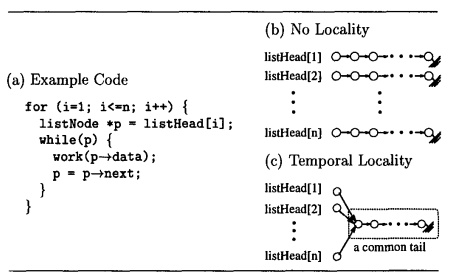
\includegraphics[width=0.6\textwidth]{p247.png}
    \caption{Example of list traversals, both with and without temporal data locality. }
    \label{fig:p247}
\end{figure}



\subsubsection{Scheduling}

Our ability to schedule prefetches for an RDS is also constrained
by the fact that nodes are linked together through pointers. For
example, consider the case shown in Figure \ref{fig:p248}(a), where assuming
that three nodes worth of computation is needed to hide the
latency, we would like to initiate a prefetch for node $n_{i+3}$  while
we are visiting node $n_i$ The problem is that to compute the
address of node $n_{i+3}$ , we must first dereference a pointer in node
$n_{i+2}$ , and to do that, we must first dereference a pointer in node
$n_{i+1}$  etc. As a result, one cannot prefetch (or fetch) a future
node until all nodes between it and the current node have been
fetched. However, the very act of touching these intermediate
nodes means that we cannot tolerate the latency of fetching more
than one node ahead. For example, the prefetching code shown
in Figure \ref{fig:p248}(b) will not hide any more latency than the code in
Figure \ref{fig:p248}(c).1 In fact, the code in Figure \ref{fig:p248}(c) is likely to run faster
since it has less instruction overhead. This example illustrates
what we refer to as the pointer-chasing problem.

Since scheduling RDS prefetches is such a difficult problem, we
make it the primary focus of this paper. Improvements in analysis tend to reduce prefetching overhead by eliminating unnecessary prefetches. However, without sufficient scheduling techniques, there will be no upside to prefetching and hence reducing
overhead will be irrelevant. Fortunately, as we discuss in the
next subsection, there are techniques for scheduling prefetches
that avoid the pointer-chasing problem.



\begin{figure}[H]
    \centering
    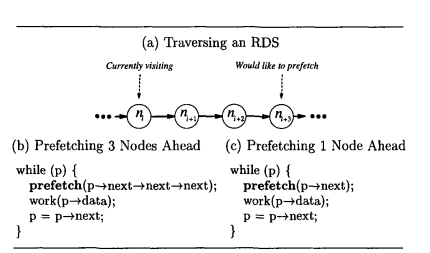
\includegraphics[width=0.6\textwidth]{p248.png}
    \caption{Illustration of the pointer-chasing problem.  }
    \label{fig:p248}
\end{figure}


\subsubsection{Greedy Prefetching}

In a k-ary RDS, each node contains k pointers to other nodes.
Greedy prefetching exploits the fact that when $k > 1$, only one
of these $k$ pointers can be immediately followed by control flow
as the next node in the traversal. Hence the remaining $k - 1$
pointers serve as natural jump-pointers, and can be prefetched
immediately upon first visiting a node. Although none of these
jump-pointers may actually point to $n_{i+d}$ , hopefully each of them
points to $n_{i+d^{\prime}}$ , for some $d^{\prime}  > 0$. If $d^{\prime} < d$, then the latency may
be partially hidden; if  > d, then we expect the latency to be
fully hidden, provided that the node is not displaced from the
cache before it is referenced (which may occur if $d^{\prime} >> d$).

To illustrate how greedy prefetching works, consider the preorder
traversal of a binary tree (i.e. $k = 2$), where Figure \ref{fig:p249}(a)
shows the code with greedy prefetching added. Assuming that
the computation in \texttt{process()} takes half as long as the cache
miss latency, we would want to prefetch two nodes ahead (i.e.
$d = 2$) to fully hide the latency. Figure \ref{fig:p249}(b) shows the caching
behavior of each node. We obviously suffer a full cache miss at
the root node (node 1), since there was no opportunity to fetch
it ahead of time. However, we would only suffer half of the miss
penalty ($\frac{L}{2}$) when we visit node 2, and no miss penalty when
we eventually visit node 3 (since the time to visit the subtree
rooted at node 2 is greater than $L$). In this example, the latency
is fully hidden for roughly half of the nodes, and reduced by
50\% for the other half (minus the root node). If we generalize
this example to a k-ary tree, we would expect the fraction of
nodes where latency is fully hidden to be roughly $\frac{k-1}{k}$(assuming
that prefetched nodes are generally not displaced from the cache
before they are referenced). Hence a larger value of $k$ is likely
to improve the performance of greedy prefetching, since more
natural jump-pointers are available.


\begin{figure}[H]
    \centering
    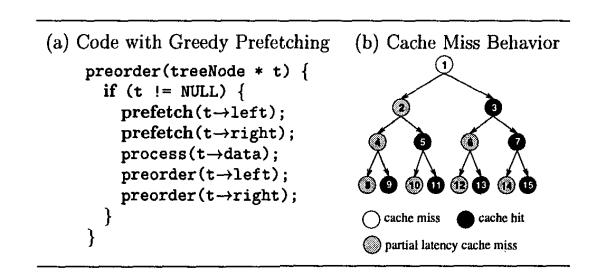
\includegraphics[width=0.6\textwidth]{p249.png}
    \caption{Illustration of greedy prefetching.  }
    \label{fig:p249}
\end{figure}


Greedy prefetching offers the following advantages:
(i) it has
low runtime overhead, since no additional storage or computation is needed to construct the natural jump-pointers;
(ii) it is
applicable to a wide variety of RDSs, regardless of how they are
accessed or whether their structure is modified frequently; and
(iii) it is relatively straightforward to implement in a compiler. The main disadvantage of greedy prefetching is that it does not offer precise control over the prefetching
distance, which is the motivation for our next algorithm.


